\section{Discussie}

% Discus the results. 
% Show what the fitting coefficient is after calculation.

In \autoref{fig:pathLossMesurment:pathloss} is het te zien dat de hoeveelheid path loss die optreed niet afhankelijk lijkt te zijn van het signaal vermogen. Dit komt ook overeen met de verschillende modellen die in \autoref{sec:introduction} zijn behandeld. Om een beter beeld te krijgen van het signaalverlies is in \autoref{fig:pathLossMesurment:avaragePathloss} de gemiddelde path loss getoond en in \autoref{fig:pathLossMesurment:medianPathloss} de  mediane path loss.
\begin{figure}[ht]
    \centering
\begin{tikzpicture}
    \begin{axis}[
        title={},
        xlabel={Afstand (m)},
        ylabel={PL (dB)},
        grid=major,
        cycle list name=color list,
        no markers,
        every axis plot/.append style={thick},
        legend pos=outer north east,
        legend style={font=\small}
    ]
    \addlegendimage{empty legend}
    \addplot table [x=Distance,y=-10] {sections/data3.dat};
    % \addlegendentry{\hspace{-.6cm}\textbf{TSS}}
    % \addlegendentry{PL}
    \end{axis}
\end{tikzpicture}

%TODO: Add better title?
\caption{Gemiddeld signaalverlies over afstand.}
\label{fig:pathLossMesurment:avaragePathloss}

\end{figure}
\begin{figure}[ht]
    \centering
\begin{tikzpicture}
    \begin{axis}[
        title={},
        xlabel={Afstand (m)},
        ylabel={PL (dB)},
        grid=major,
        cycle list name=color list,
        no markers,
        every axis plot/.append style={thick},
        legend pos=outer north east,
        legend style={font=\small}
    ]
    \addlegendimage{empty legend}
    \addplot table [x=Distance,y=5] {sections/data4.dat};
    % \addlegendentry{\hspace{-.6cm}\textbf{TSS}}
    % \addlegendentry{PL}
    \end{axis}
\end{tikzpicture}

%TODO: Add better title?
\caption{De mediaan van het signaalverlies over afstand.}
\label{fig:pathLossMesurment:medianPathloss}

\end{figure}

Om te controleren of de gemeten data overeen komt met de modellen uit \autoref{sec:introduction}, is in \autoref{fig:modelPredictions} de verwachting van verschillende modellen geplot. Hierbij is voor $\epsilon_r$ een waarde van 3.4 gebruikt. Deze $\epsilon_r$ komt overeen met de $\epsilon_r$ van beton bestaande uit kleine korrels \cite{zhekov2020dielectric}.
\begin{figure}[ht]
    \centering
    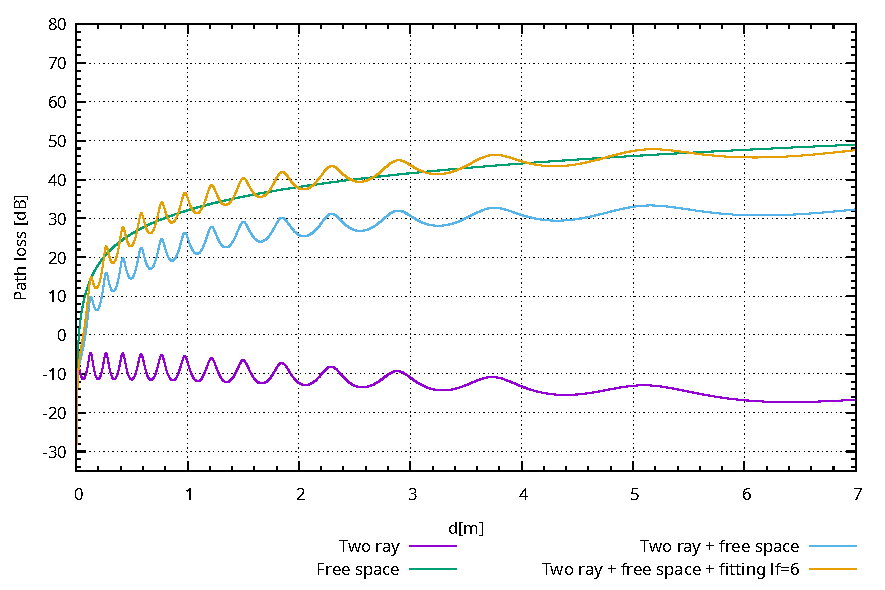
\includegraphics[width=0.8\textwidth]{twoRayModelPlot}
    \caption{Verwachte path loss van verschillende modellen}
    \label{fig:modelPredictions}
\end{figure}

Om uit de meetdata informatie te halen over de fittingscoëfficiënt wordt \autoref{eq:calcfittingsCoef} gebruikt. In \autoref{fig:pathLossMesurment:fittingscoef} is te zien wat de fittingscoëfficiënt is voor de gemeten path loss waardes. De gemiddelde fittingscoëfficiënt van de metingen komt uit op 7.71 en de mediane fittingscoëfficiënt komt uit op 7.80.
\begin{equation} \label{eq:calcfittingsCoef}
    l_f=\frac{PL-PL_{FS}-PL_{TR}}{\log\left(50d\right)}
\end{equation}
\begin{figure}[ht]
    \centering
\begin{tikzpicture}
    \begin{axis}[
        title={},
        xlabel={Afstand (m)},
        ylabel={fittingscoëfficiënt},
        grid=major,
        cycle list name=color list,
        no markers,
        every axis plot/.append style={thick},
        legend pos=outer north east,
        legend style={font=\small}
    ]
    \addlegendimage{empty legend}
    \addplot table [x=Distance,y=median] {sections/data5.dat};
    \addplot table [x=Distance,y=average] {sections/data5.dat};
    \addlegendentry{\hspace{-.6cm}\textbf{fittingscoëfficiënt}}
    \addlegendentry{mediaan}
    \addlegendentry{gemiddelde}
    \end{axis}
\end{tikzpicture}
\caption{De mediaan van het signaalverlies over afstand.}
\label{fig:pathLossMesurment:fittingscoef}
\end{figure}

\subsection{Mogelijke bronnen van fouten}
Het is duidelijk dat de gemeten fittingscoëfficiënt erg van waarde verandert over afstand. Dit kan door verschillende dingen komen. Bij het meten is het ontvangstvermogen met de hand afgelezen. Hierbij is op te merken dat de ontvangstvermogenswaarde die op de spectrumanalyzer af te lezen was erg veel veranderde over tijd. Doordat er maar een enkele waarde per vermogen per afstand is afgelezen kan dit onbedoeld tot een dergelijke fout leiden.

Een ander mogelijk is dat de metingen verstoord zijn doordat er mensen langs de testopstelling zijn gelopen terwijl er werd gemeten. Dit leek tijdens het doen van de metingen een redelijke invloed te hebben op de meetresultaten.

Als derde bron van fouten was de ondergrond niet van beton maar van lag er een tapijt. Dit zorgt er voor dat de gekozen $\epsilon_r$ in dit meetrapport niet de goede waarde heeft. Naast dat de $\epsilon_r$ mogelijk fout is heeft dit ook een invloed op hoe de elektromagnetische golven weerkaatsen op een oppervlak. 

\subsection{Aanbevelingen}
Voor een vervolg meeting wordt het aangeraden om meer samples te nemen per afstand per vermogen. Ook wordt het aangeraden om de afstand tussen de antennes met kleinere stappen te vergroten.

Een andere richting van interesse voor vervolg onderzoek kan het volgende zijn: het onderzoeken van het effect van het plafond. Wanneer kan het effect van een plafond worden verwaarloosd en wanneer kunnen de effecten van het plafond niet worden verwaarloosd.